\section{Results and Discussion}
\label{sec:results}

\subsection{Detection Accuracy}
\label{sec:res_detection}
Table~\ref{tab:accuracy_results} summarizes accuracy after identical 20-epoch budgets, and Fig.~\ref{fig:convergence_map} shows the validation curves. Two views must be distinguished. At the \emph{final epoch}, the baseline leads with $69.75\%\ \text{mAP}_{50}$, ahead of Arm~4 ($67.17\%$), Arm~3 ($67.10\%$), and Arm~2 ($65.46\%$), and with $45.83\%\ \text{mAP}_{50-95}$ versus $41.56$--$43.17\%$. At the \emph{best-fitness checkpoint}, Arm~2 reaches $71.95\%$ (epoch 18) versus $69.80\%$ for the baseline (epoch 20), but this checkpoint is selected on the same $100$ frames on which it is reported, so the figure is optimistically biased and we do not interpret it as evidence for SS2D. All SS2D arms have lower $\text{mAP}_{50-95}$ under either view. Validation $\text{mAP}_{50}$ also changes by up to $14$ points between consecutive epochs after epoch $5$, and by up to $33$ points in the first epochs of Arm~4, which exceeds the $+2.15$-point gap between Arm~2 and the baseline; switching off mosaic at epoch $11$ may contribute. With a single seed, differences between arms cannot be distinguished from run-to-run variance.

\begin{table}[t]
\caption{Accuracy on the validation partition (single seed). Best-fitness checkpoints are selected on the same partition and are therefore optimistically biased; P and R refer to them, the box loss to the final epoch. Arm~3 epochs are counted within stage~2. Final-epoch values come from the validation run during training, best-fitness values from a standalone re-validation of \texttt{best.pt}; for Arms~1 and~4, whose best checkpoint is the final epoch, the two differ by at most $0.3$ points.}
\label{tab:accuracy_results}
\centering
\footnotesize
\setlength{\tabcolsep}{2.6pt}
\begin{tabular}{lccccccc}
\toprule
 & \multicolumn{2}{c}{\textbf{Final epoch}} & \multicolumn{2}{c}{\textbf{Best fitness}} & & & \textbf{Final val.} \\
\cmidrule(lr){2-3} \cmidrule(lr){4-5}
\textbf{Arm} & $\textbf{mAP}_{50}$ & $\textbf{mAP}_{50-95}$ & $\textbf{mAP}_{50}$ (ep.) & $\textbf{mAP}_{50-95}$ & \textbf{P} & \textbf{R} & \textbf{box loss} \\
\midrule
1: Baseline & \textbf{69.75} & \textbf{45.83} & 69.80 (20) & \textbf{45.53} & \textbf{0.818} & 0.572 & \textbf{1.0196} \\
2: SS2D, single-stage & 65.46 & 41.56 & \textbf{71.95} (18) & 45.15 & 0.744 & 0.576 & 1.0688 \\
3: SS2D, two-stage & 67.10 & 43.17 & 67.67 (14) & 43.15 & 0.741 & \textbf{0.651} & 1.0512 \\
4: SS2D, dual-scale & 67.17 & 42.73 & 67.17 (20) & 42.76 & 0.738 & 0.515 & 1.0863 \\
\bottomrule
\end{tabular}
\end{table}

\begin{figure}[t]
\centering
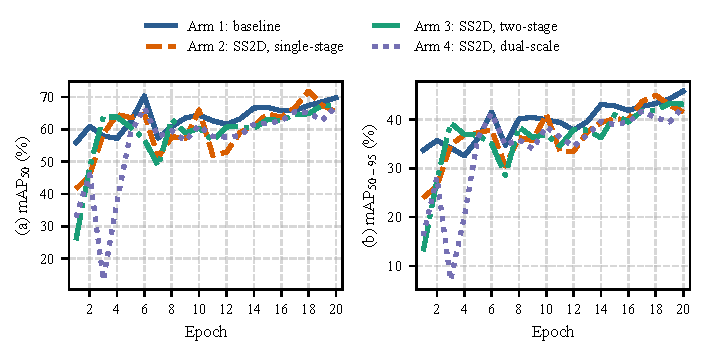
\includegraphics[width=\textwidth]{figures/fig_convergence_map_wide.pdf}
\caption{Validation (a) $\text{mAP}_{50}$ and (b) $\text{mAP}_{50-95}$ over 20 epochs (one seed per arm, so no run-to-run variance is shown). For Arm~3, epochs 1--5 are stage~1 and epochs 6--20 are stage-2 epochs 1--15, so its best-fitness checkpoint (stage-2 epoch 14) appears at epoch 19.}
\label{fig:convergence_map}
\end{figure}

Two-stage training (Arm~3) has the highest recall ($0.651$ vs.\ $0.572$ for the baseline) but lower precision ($0.741$ vs.\ $0.818$). Because both are reported at the F1-maximizing threshold, this is mainly a shift of the operating point: the derived F1 is $0.693$ vs.\ $0.673$, and $0.683$ vs.\ $0.673$ at the final epoch. The dual-scale model (Arm~4) is close to Arm~3, so adding a $P_4$ block brings no measurable benefit here at a substantial runtime cost. In an initial version of the SS2D pipeline, adapting the COCO head to four classes also re-initialized the $42$ class-agnostic box-regression tensors, raising the initial box loss to $6.276$; transferring all shape-compatible tensors, as Ultralytics does for the baseline, lowers it to $2.758$, and all reported SS2D models use this correction.

\begin{table}[t]
\caption{Per-class $\text{mAP}_{50}$ / $\text{mAP}_{50-95}$ (\%) of the best-fitness checkpoints on the validation partition (also used for checkpoint selection).}
\label{tab:per_class_results}
\centering
\footnotesize
\setlength{\tabcolsep}{4pt}
\begin{tabular}{lcccc}
\toprule
\textbf{Class (val.\ instances)} & \textbf{Arm 1} & \textbf{Arm 2} & \textbf{Arm 3} & \textbf{Arm 4} \\
\midrule
\texttt{worker} ($3{,}488$) & 89.2 / \textbf{63.2} & \textbf{89.4} / 61.9 & 87.9 / 60.5 & 88.5 / 60.9 \\
\texttt{forklift} ($150$) & 70.1 / 31.8 & \textbf{79.7} / 38.3 & 76.3 / \textbf{38.4} & 75.3 / 33.8 \\
\texttt{pallet\_truck}$^{\dagger}$ ($13$) & 32.8 / \textbf{22.4} & \textbf{33.9} / 17.7 & 22.9 / 16.2 & 20.0 / 14.6 \\
\texttt{amr} ($45$) & \textbf{87.1} / \textbf{64.7} & 84.9 / 62.6 & 83.7 / 57.5 & 85.0 / 61.7 \\
\midrule
Macro (4 classes) & 69.80 / \textbf{45.53} & \textbf{71.95} / 45.15 & 67.67 / 43.15 & 67.17 / 42.76 \\
Macro (3 classes)$^{\ddagger}$ & 82.1 / 53.2 & \textbf{84.7} / \textbf{54.3} & 82.6 / 52.1 & 82.9 / 52.1 \\
\bottomrule
\multicolumn{5}{p{0.92\textwidth}}{\scriptsize $^{\dagger}$Only $13$ validation instances ($0.35\%$ of labels); not interpreted. $^{\ddagger}$Without \texttt{pallet\_truck}, from the rounded per-class values.} \\
\end{tabular}
\end{table}

Per class (Table~\ref{tab:per_class_results}), all SS2D arms score above the baseline on the $150$ forklift instances ($75.3$--$79.7\%$ vs.\ $70.1\%\ \text{mAP}_{50}$, and $+2.0$ to $+6.6$ points in $\text{mAP}_{50-95}$), the largest and most consistent difference; without \texttt{pallet\_truck}, the best-fitness checkpoint of Arm~2 also leads in macro $\text{mAP}_{50-95}$ ($54.3$ vs.\ $53.2$), a view that is selection-biased in the same way. Forklifts are also the largest objects in the validation partition: their mean box area is $0.0274$ of the image, versus $0.0093$ for workers and $0.0027$ for AMRs, i.e.\ about $2.5$, $1.4$, and $0.8$ cells of the stride-32 $P_5$ grid on a side. Larger objects may depend more on the deep features where the two models differ, but this is a hypothesis, not an explanation: \texttt{C2PSA} attends over all $400$ $P_5$ positions whereas the trained scan mixes mostly locally (Section~\ref{sec:mamba_integration}), the comparison covers one seed and four classes, and without trained identity or convolution-only replacements the difference cannot be attributed to the selective scan rather than to the removal of \texttt{C2PSA} or to variance. The $150$ instances also come from $100$ frames of two cameras, so the number of distinct forklifts is much smaller; the difference has yet to be tested across seeds and with a track-level bootstrap. Workers change little in $\text{mAP}_{50}$ ($87.9$--$89.4\%$) but are lower in $\text{mAP}_{50-95}$ for all SS2D arms, and AMRs are slightly lower ($83.7$--$85.0\%$ vs.\ $87.1\%$). Fig.~\ref{fig:qualitative_comparison} illustrates the mixed picture on one dense frame (\texttt{f000360}, the second most crowded of the $100$ validation frames with $57$ objects versus a median of $26$, and one that contains all four classes): the baseline finds $46$ of $57$ objects with $2$ false positives, Arm~2 finds $42$ with $8$, and Arm~3 finds $44$ with $4$.

\begin{figure}[t]
\centering
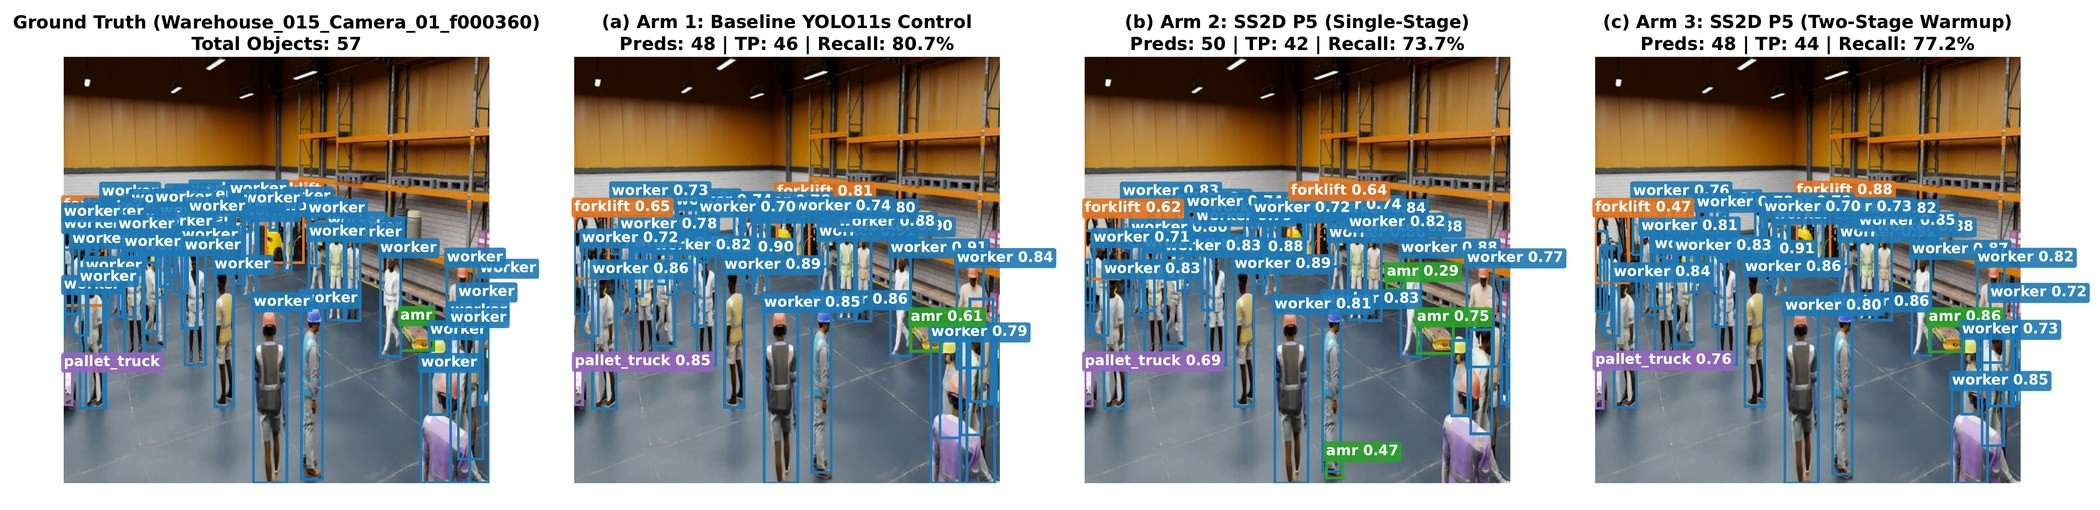
\includegraphics[width=\textwidth]{figures/fig_qualitative_f000360.jpg}
\caption{Predictions on validation frame \texttt{f000360} (\texttt{Warehouse\_015}, \texttt{Camera\_01}): ground truth, Arm~1, Arm~2, and Arm~3 (best-fitness checkpoints, confidence $\ge 0.25$, NMS IoU $0.45$), with the number of predictions, true positives (same class, $\text{IoU} \ge 0.5$, one match per ground-truth box), and recall.}
\label{fig:qualitative_comparison}
\end{figure}

\subsection{Edge Deployment}
\label{sec:res_edge}
Static savings do not carry over to deployment. Although SS2D-P5 has $0.63$\,M fewer parameters ($2.4$\,MiB in FP32), its ONNX file is larger ($38.5$ vs.\ $36.2$\,MiB) because the unrolled graph stores per-step constants (the same weights exported as a parallel scan take $34.7$\,MiB), and Table~\ref{tab:edge_runtime} shows that on the Cortex-A72 it is slower than the baseline by $5.7\%$ with one thread and $17.6\%$ with four threads. Its peak memory on the Pi is $373.6$\,MiB, $63.5\%$ below a $1$\,GiB budget but $60.1\%$ above the baseline ($233.4$\,MiB); SS2D-P4P5 peaks at $718.3$\,MiB. With four threads the Pi reaches $0.76$\,FPS for SS2D-P5, $0.52$\,FPS for SS2D-P4P5, and $0.90$\,FPS for the baseline, excluding preprocessing and NMS; the CPU results therefore establish operator portability and fit within $1$\,GiB, not real-time capability.

\begin{table}[t]
\caption{ONNX Runtime forward-pass latency and memory on the Raspberry Pi~4 ($640 \times 640$, batch size 1, FP32). Mem.: peak RSS. Rel.: median relative to the baseline of the same session and thread count.}
\label{tab:edge_runtime}
\centering
\footnotesize
\setlength{\tabcolsep}{3pt}
\begin{tabular}{llccccc}
\toprule
\textbf{Model} & \textbf{Threads} & \textbf{Mem.\ (MiB)} & \textbf{Median (ms)} & \textbf{Mean $\pm$ SD (ms)} & \textbf{Rel.} & \textbf{FPS} \\
\midrule
\multicolumn{7}{l}{\textit{Session~2 (100 calls with 1 thread, 30 with 4)}} \\
Baseline & 1 & 233.2 & 3192.88 & 3194.63 $\pm$ 5.0 & 1.00 & 0.31 \\
SS2D-P5 & 1 & 373.1 & 3374.10 & 3374.58 $\pm$ 3.6 & 1.06 & 0.30 \\
Baseline & 4 & 233.4 & 1117.27 & 1120.62 $\pm$ 7.5 & 1.00 & 0.90 \\
SS2D-P5 & 4 & 373.6 & 1314.26 & 1316.11 $\pm$ 4.8 & 1.18 & 0.76 \\
\midrule
\multicolumn{7}{l}{\textit{Session~1 (100 calls with 1 thread, 30 with 4)}} \\
Baseline & 1 & 233.2 & 3360.50 & 3360.15 $\pm$ 5.2 & 1.00 & 0.30 \\
SS2D-P4P5 & 1 & 716.5 & 4178.68 & 4178.96 $\pm$ 3.5 & 1.24 & 0.24 \\
Baseline & 4 & 233.3 & 1106.76 & 1110.09 $\pm$ 7.3 & 1.00 & 0.90 \\
SS2D-P4P5 & 4 & 718.3 & 1927.71 & 1929.04 $\pm$ 7.7 & 1.74 & 0.52 \\
\bottomrule
\multicolumn{7}{p{0.95\textwidth}}{\scriptsize Relative to session~2, the session-1 baseline median is $5.2\%$ higher with one thread (the clock of the session-1 single-thread runs was not logged) and $0.9\%$ lower with four threads.} \\
\end{tabular}
\end{table}

\textbf{Why the cheaper model is slower.} Table~\ref{tab:graph_profile} points to the scan's many small operators. (1)~Exporting the four-direction scan unrolls its loop over $L = 400$ steps into $14{,}771$ ONNX nodes ($4{,}800$ \texttt{Gather}, $3{,}293$ \texttt{Mul}, $3{,}212$ \texttt{Unsqueeze}, $1{,}621$ \texttt{Add}, $1{,}600$ \texttt{ReduceSum}), versus $320$ for the baseline; ONNX Runtime removes only $70$ of them. SS2D-P4P5 has $90{,}201$ nodes. (2)~Convolution time per call is nearly constant ($905$, $865$, and $877$\,ms), but its share of kernel time falls from $78.4\%$ to $50.0\%$ (SS2D-P5) and $22.5\%$ (SS2D-P4P5), while the scan's element-wise and indexing operators take $35.1\%$ and $68.4\%$. The profiler's per-node overhead (mean profiled call $1161$, $1951$, and $4943$\,ms) inflates these shares; the constant convolution time is more robust. With the small analytical cost of the scan (Section~\ref{sec:complexity}), this indicates that the extra latency comes from the operators executed per call rather than from arithmetic. (3)~Going from one to four threads speeds up the baseline by $2.86\times$ but SS2D-P5 by only $2.57\times$ (session~2), and the baseline by $3.04\times$ but SS2D-P4P5 by $2.17\times$ (session~1), consistent with a long chain of small dependent operators that leave little work to parallelize.

\begin{table}[t]
\caption{ONNX graph size and operator profile on the Pi (four threads, five profiled calls). Conv/scan: share of summed kernel time taken by convolutions and by the scan operators (\texttt{Mul}, \texttt{Squeeze}, \texttt{Unsqueeze}, \texttt{Add}, \texttt{ReduceSum}, \texttt{Gather}, \texttt{Split}).}
\label{tab:graph_profile}
\centering
\footnotesize
\setlength{\tabcolsep}{3.4pt}
\begin{tabular}{lccccc}
\toprule
\textbf{Model} & \textbf{Nodes} & \textbf{After ORT opt.} & \textbf{ONNX (MiB)} & \textbf{Conv (ms/call)} & \textbf{Conv / scan (\%)} \\
\midrule
Baseline & 320 & 236 & 36.2 & 905 & 78.4 / $<2.5$ \\
SS2D-P5 & 14{,}771 & 14{,}701 & 38.5 & 865 & 50.0 / 35.1 \\
SS2D-P4P5 & 90{,}201 & 72{,}385 & 46.6 & 877 & 22.5 / 68.4 \\
\bottomrule
\multicolumn{6}{p{0.92\textwidth}}{\scriptsize Baseline and SS2D-P4P5 profiled in session~1 without a clock log, SS2D-P5 in session~2 at $1.5$\,GHz.} \\
\end{tabular}
\end{table}

\textbf{Runtime intervention.} These observations are correlational, so we changed the graph form of the scan while keeping its computation fixed (Table~\ref{tab:g1_intervention}). First, removing the $P_5$ block entirely lowers latency by only $2.4\%$ (one thread) and $5.3\%$ (four threads), and the convolution-only block costs about the same, whereas the SS2D block adds $17.0\%$ and $22.2\%$ over the identity model. Second, fewer nodes did not mean lower latency: one ONNX \texttt{Loop} per direction shrinks the graph from $14{,}767$ to $367$ nodes but makes the model $2.2\times$ and $4.5\times$ slower than the unrolled scan, because its $37$--$38$-node body runs $400$ times per direction, about $60{,}000$ node executions per call. The chunked scan cuts the graph by $43\%$ but adds computation within each chunk and is $4.4\%$ and $14.0\%$ slower. Third, removing the dependency chain did not help either: a parallel associative scan~\cite{blelloch1990prefix} evaluates the same recurrence in $\lceil \log_2 L \rceil = 9$ whole-sequence steps with $619$ nodes (about $540$ after ONNX Runtime graph optimization, mostly \texttt{Mul}, \texttt{Slice}, \texttt{Pad}, and \texttt{Add}; no fused scan kernel), yet with the trained Arm~3 weights it is $20\%$ (one thread) and $64\%$ (four threads) slower than the unrolled export, and its one-to-four-thread speed-up drops to $1.81\times$ (baseline $2.73\times$, unrolled $2.48\times$). Fourth, removing arithmetic did not help: computing $\mathbf{W}_{\text{proj}}$ once removes $88.5$ of the $131.1$\,M MACs of the scan core, yet the export is $0.3\%$ (one thread) and $2.7\%$ (four threads) slower than the unrolled one. Neither node count, the sequential chain, nor the core's arithmetic is thus the cause on its own; the two forms pay different costs for the same small arithmetic ($13.1$\,M MACs). The unrolled scan executes a long chain of small dependent operators, whereas the parallel scan repeatedly reads and writes the full $400 \times 256 \times 16$ state of each direction ($6.25$\,MiB per tensor). Hardware counters (\texttt{perf stat}, one thread) support both: against the unrolled scan, the parallel scan retires $7\%$ more instructions but takes $25\%$ more cycles (IPC $0.76$ vs.\ $0.89$) with $2.2\times$ the estimated DRAM traffic, while the unrolled scan retires $10\%$ more instructions than the baseline at the same IPC. Fused kernels and the matrix (SSD) form of Mamba-2~\cite{dao2024mamba2}, which requires a scalar decay per head and thus a modified, retrained block, remain untested. The untrained upper block is not comparable with Table~\ref{tab:edge_runtime} in absolute terms (one-thread offset $6.5\%$). Only within-session ratios are interpreted (the session-4 baseline is up to $4.9\%$ off session~2); they reproduce the SS2D-P5 overhead of Table~\ref{tab:edge_runtime} ($1.06\times$ and $1.17\times$). Creating a session for the unrolled graph also takes $46$--$47$\,s (one or four threads), against $0.3$--$0.5$\,s for the baseline and the parallel scan.

\begin{table}[t]
\caption{Runtime intervention on the Pi: median latency in ms; Rel.: relative to the baseline of the same block at the same thread count; MiB: peak RSS with four threads. Upper block: session~2, untrained exports, 3 warmup and 20 timed calls (SD at most $10.8$\,ms). Lower block: session~4, trained Arm~1 and Arm~3 exports, protocol of Table~\ref{tab:edge_runtime} (SD at most $26.0$\,ms).}
\label{tab:g1_intervention}
\centering
\footnotesize
\setlength{\tabcolsep}{5pt}
\begin{tabular}{lcccccc}
\toprule
\textbf{Variant} & \textbf{Nodes} & \textbf{1 thread} & \textbf{Rel.} & \textbf{4 threads} & \textbf{Rel.} & \textbf{MiB} \\
\midrule
Baseline (\texttt{C2PSA}) & 320 & 3146.7 & 1.00 & 1132.8 & 1.00 & 233.3 \\
$P_5$ block removed & 292 & 3070.4 & 0.98 & 1072.7 & 0.95 & 229.4 \\
Convolution-only & 300 & 3105.4 & 0.99 & 1095.9 & 0.97 & 230.5 \\
SS2D, unrolled & 14{,}767 & 3593.8 & 1.14 & 1311.3 & 1.16 & 373.6 \\
SS2D, ONNX \texttt{Loop} & 367 & 7778.6 & 2.47 & 5938.4 & 5.24 & 274.0 \\
SS2D, chunked ($T = 4$) & 8{,}355 & 3752.5 & 1.19 & 1494.7 & 1.32 & 304.3 \\
\midrule
\multicolumn{7}{l}{\textit{Trained exports, session~4}} \\
Baseline (\texttt{C2PSA}) & 320 & 3204.1 & 1.00 & 1171.8 & 1.00 & 233.4 \\
SS2D, unrolled & 14{,}771 & 3396.6 & 1.06 & 1370.8 & 1.17 & 373.6 \\
SS2D, $\mathbf{W}_{\text{proj}}$ once & 14{,}773 & 3407.0 & 1.06 & 1407.4 & 1.20 & 374.1 \\
SS2D, parallel scan & 619 & 4089.6 & 1.28 & 2253.6 & 1.92 & 389.6 \\
\bottomrule
\multicolumn{7}{p{0.92\textwidth}}{\scriptsize Session creation with four threads: $0.26$\,s (baseline), $47.3$\,s (unrolled), $44.7$\,s ($\mathbf{W}_{\text{proj}}$ once), $0.34$\,s (parallel scan).} \\
\end{tabular}
\end{table}

\subsection{Design Lessons and Limitations}
\label{sec:limitations}
Three lessons follow for replacing attention with selective scans in small detectors. (1)~\emph{Fewer FLOPs can mean a slower model}, and neither a smaller graph, a parallel scan, nor less arithmetic necessarily helps on a CPU; latency and memory should be measured at the deployed thread count. (2)~\emph{Comparisons need identical warm starts}: the class-agnostic box-regression branch must be transferred for every arm. In a two-epoch pilot with an earlier version of the block, in which this branch was not transferred, the SS2D model reached $0.09\%$ $\text{mAP}_{50}$ against $39.8\%$ for the baseline (training box loss $4.50$ vs.\ $1.30$); all reported arms transfer it. (3)~\emph{A zero-initialized convolution ahead of BN is not an identity initialization}; zero-$\gamma$ initialization (Eq.~\eqref{eq:zero_gamma}) avoids the problem by construction, although its effect on detector training remains to be measured.

The results have clear limitations. All accuracy results come from one seed, a 20-epoch budget, and one $100$-frame validation facility that also served for checkpoint selection, without a held-out test facility or significance testing. The data are synthetic, cover two facilities, and consecutive frames are highly correlated. The reported SS2D models use the initialization of Eq.~\eqref{eq:zero_wout}, and because Arm~3 combines freezing with a restarted schedule, its differences from Arm~2 cannot be attributed to either factor alone. Identity and convolution-only replacements were measured for runtime only, so no trained ablation separates the scan from the removal of \texttt{C2PSA}, and the simplifications relative to Mamba are not ablated. Edge measurements cover only the forward pass on one embedded CPU in FP32; preprocessing, NMS, the session creation of SS2D-P4P5 (tens of minutes, not timed), accelerators, quantization, and energy were not measured. The Pi results come from five sessions, and most intervention variants use untrained exports.
